% 介质中的静电场
% 极化强度|极化电荷|极化率|介电常量|电容率

\pentry{电极化强度与极化电荷的关系\upref{ElePAP}}

如果把激发外电场的原有电荷系称为自由电荷,并用$\mathbf E_0$表示它们所激发的电场强度,而用$\mathbf E'$表示极化过程完成之后极化电荷所激发的电场强度.那么,空间任一点最终的合电场强度$\mathbf E $应是上述两类电荷所激发电场强度的矢量和,即
\begin{equation}
\bvec E = \bvec E_{0} + \bvec E'
\end{equation}
由于在电介质中,自由电荷的电场与极化电荷的电场的方向总是相反,所以在电介质中的合电场强度$\mathbf E $与外电场强度$\mathbf E_0$相比显著地削弱了.

对于各向同性线性电介质,电极化强度$\mathbf P $和介质内部的合电场强度$\mathbf E $的关系为
\begin{equation} 
\mathbf P=\chi_{\mathrm e} \varepsilon_{0} \mathbf E
\end{equation}
式中的比例因数$\chi_{\mathrm{e}}$和电介质的性质有关,叫做电介质的\textbf{电极化率(electric susceptibility)},是量纲为$1 $的量.

\begin{figure}[ht]
\centering
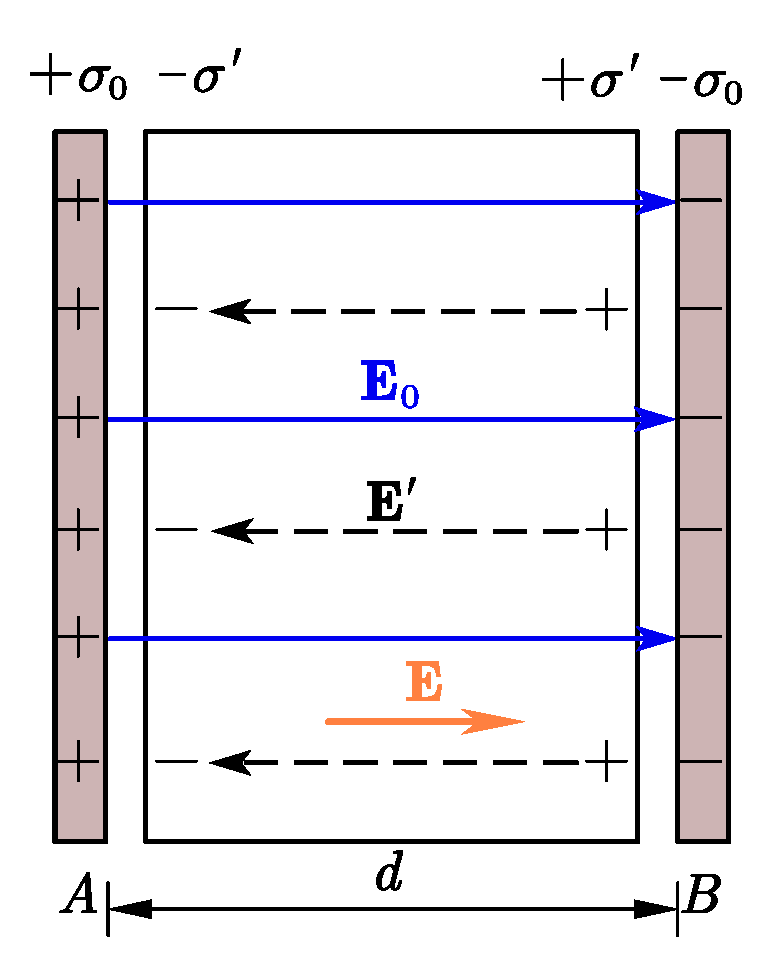
\includegraphics[width=6cm]{./figures/EFIDE_1.pdf}
\caption{电介质中的电场强度} \label{EFIDE_fig1}
\end{figure}
为了定量地了解电介质内部电场强度被削弱的情况,我们讨论如下特例:\autoref{EFIDE_fig1}表示在两块“无限大”极板间充有电极化率为$\chi_\mathrm{e}$的均匀电介质,设两极板上的自由电荷面密度为$\pm \sigma_0$,电介质表面上的极化电荷面密度为$\pm \sigma^\prime$.自由电荷的电场强度大小$E_{0}=\sigma_{0} / \varepsilon_{0}$,在图中用实线表示;极化电荷的电场强度大小为$E^{\prime}=\sigma^{\prime} / \varepsilon_{0}$,在图中用虚线表示.$\mathbf E^\prime$的方向和$\mathbf E_0$的方向相反,因此极板间电介质中的合电场强度$\mathbf E $的大小为
\begin{equation}
E=E_{0}-E^{\prime}=\frac{\sigma_{0}}{\varepsilon_{0}}-\frac{\sigma^{\prime}}{\varepsilon_{0}}
\end{equation}
考虑到极化电荷面密度为$\sigma$,极板间电介质中的合电场强度$\mathbf E $的大小又可写为
\begin{equation}
E=E_{0}-\frac{P}{\varepsilon_{0}}=E_{0}-\chi_{\mathrm e} E
\end{equation}
即
\begin{equation} \label{EFIDE_eq1}
E=\frac{E_{0}}{1+\chi_{\mathrm{e}}}
\end{equation}
说明电介质内部的电场强度$E $被削弱为外电场强度$E_0$的${1+\chi_{\mathrm{e}}}$.下面我们将看到$({1+\chi_{\mathrm{e}}})$正是电介质的相对电容率$\varepsilon_\mathrm{r}$.我们知道,两极板间的电势差为
\begin{equation}
U=E d=\frac{\sigma_{0} d}{\varepsilon_{0}\left(1+\chi_{\mathrm e}\right)}
\end{equation}
设极板的面积为$S$,则极板上总的电荷量为$q=\sigma_{0} S$,按电容器电容的定义,极板间充满均匀电介质后的电容为
\begin{equation}
C=\frac{q}{U}=\frac{\varepsilon_{0}\left(1+\chi_{\mathrm e}\right) S}{d}=\left(1+\chi_{\mathrm e}\right) C_{0}
\end{equation}
而我们知道$C=\varepsilon_\mathrm{r}C_0$,所以
\begin{equation} \label{EFIDE_eq2}
\varepsilon_{\mathrm{r}}=1+\chi_{\mathrm{e}}
\end{equation}
这就解释了电容器中充满电介质后其电容增大的实验事实.又令
\begin{equation}
\varepsilon=\varepsilon_{r} \varepsilon_{0}=\left(1+\chi_{\mathrm{e}}\right) \varepsilon_{0}
\end{equation}
称作电介质的\textbf{电容率}或\textbf{介电常量}.与真空中的电容率$\varepsilon_0$有相同的单位.电极化率$\chi_{\mathrm{e}}$、相对电容率$\varepsilon_\mathrm{r}$,和电容率$\varepsilon$都是表征电介质性质的物理量,三者中知道任何一个即可求得其他两个.

这里要特别说明一点,\autoref{EFIDE_eq2}虽然是从平行板电容器中均匀电介质的特例引出的,但它却是普遍适用的.
而\autoref{EFIDE_eq1}表明,在均匀电介质充满整个电场的情况下,电介质内部的电场强度$E $为电场强度$E_0$的$1/\varepsilon_{\mathrm{r}}$倍,这一结论并不是普遍成立的,但电介质内部的电场强度通常要减弱,这个现象却是普遍成立的.

此外做一个小扩展,上面研究的是各向同性电介质,电极化率和电容率都是常量,但自然界也存在一些电介质,在一定的温度范围内电容率随电场强度而变化,它们的极化规律有着复杂的非线性关系.例如钛酸钡等,在外电场撤除后仍保留有剩余的极化,这样的材料称作\textbf{铁电体},另一类电介质在外力的作用下发生机械变形(拉伸或压缩)时,也能产生电极化现象,称作\textbf{压电效应}.如石英晶体等就具有压电效应.压电效应的反效应叫做电致伸缩,即晶体在电场中会产生伸长或收缩的效应.还有一类材料在外电场撤销后,会长期保留其极化状态,就像永磁体保留有磁性一样.这样的电介质称作\textbf{永驻体}.上述这些具有特殊性质的材料有着重要的应用,可以制成各种换能器和传感器,满足人们不同的需求.它们是材料科学的基础研究内容之一.
